\documentclass{beamer}
\usepackage[utf8]{inputenc}
\usepackage[english]{babel}
\usepackage{helvet}
\usepackage[T1]{fontenc}
\usepackage[inline]{asymptote}
\usepackage{asy_helper}
\usepackage{slide_helper}
\usepackage{multirow}
\usepackage{cancel}
\usepackage{tikz}
\usetikzlibrary{shapes.geometric, arrows}
\usepackage{pgfplots}
\pgfplotsset{compat=1.5} 
\usepgfplotslibrary{statistics}
\usetikzlibrary{external}
\tikzexternalize%

\begin{asydef}
  import gsl;
  
  real nd_func(real mu, real sigma, real x)
  {
    return 1/sqrt(2*pi*sigma*sigma)*exp((-1*(x-mu)*(x-mu))/(2*sigma*sigma));
  }
  
  guide normal_dist(real mu, real sigma, real xmin, real xmax)
  {
    real nd(real x) { return nd_func(mu, sigma, x); }
    return graph(nd, xmin, xmax);
  }

  guide t_dist(real df, real xmin, real xmax)
  {
    real f(real x) { return pdf_tdist(x, df); }
    return graph(f, xmin, xmax);
  }

  void shade_below(real df, real b, real xmin, real xmax, pen p=royalblue)
  {
    real t_func(real x) { return pdf_tdist(x, df);}
    
    guide g = graph(t_func, xmin, b);
    
    filldraw(g -- (b,0) -- (xmin,0) --  cycle, p, black);
    
    draw((xmin,0)--(b,0));
  }

  void shade_above(real df, real b, real xmin, real xmax, pen p=royalblue)
  {
    real t_func(real x) { return pdf_tdist(x, df);}
    
    guide g = graph(t_func, b, xmax);
    
    filldraw(g -- (xmax,0) -- (b,0) -- cycle, p, black);
    
    draw((xmax,0)--(b,0));
  }
\end{asydef}

\newcommand{\satisfied}[0]{{\color{green!70!black}\checkmark}}

\title[MA205 - Section 7.1]{One-sample means with the $t$-distribution}

\newcommand{\prob}[1]{P\left({#1}\right)}
\newcommand{\jointprob}[3]{\prob{{#1}~\text{#2}~{#3}}}
\newcommand{\condprob}[2]{\prob{{#1}~|~{#2}}}
\newcommand{\comb}[2]{_{#1}C_{#2}}

\begin{document}
\begin{frame}
  \titlepage
\end{frame}

\begin{frame}
  \begin{block}{Central Limit Theorem for the Sample Mean}
    When we collect a sufficiently large sample of $n$ independent observations from a population with mean $\mu$ and standard deviation $\sigma$, the sampling distribution of $\bar{x}$ will be nearly normal with:
    \begin{equation*}
      \begin{aligned}
        \text{Mean} = \mu
        \qquad\qquad
        \text{Standard Deviation ($SE$)} = \dfrac{\sigma}{\sqrt{n}}
      \end{aligned}
    \end{equation*}
  \end{block}\pause

  \begin{note}
    It's rare to need to estimate the population mean $\mu$, but somehow know the population standard deviation $\sigma$. In most cases $\sigma$ will need to be estimated.
  \end{note}
\end{frame}

\begin{frame}
  \begin{block}{Conditions to Apply the Central Limit Theorem}
    \begin{description}
    \item[Independence:] The sample observations must be independent.\pause
    \item[Normality:] When a sample is small, we also require that the sample observations come from a normally distributed population.\pause
      \begin{description}
      \item[$\boldsymbol{n<30}$:] If the sample size $n$ is less than 30 and there are no clear outliers in the data, then we typically assume the data is from a nearly normal population.\pause
      \item[$\boldsymbol{n\geq30}$:] If the sample size $n$ is at least 30 and there are no \emph{particularly extreme outliers}, then we typically assume the sampling distribution of $\bar{x}$ is nearly normal, even if the underlying population is not.
      \end{description}
    \end{description}
  \end{block}\pause
  
  \begin{note}
    In a first course in statistics, you aren't expected to develop perfect judgment on the normality condition.
  \end{note}
\end{frame}

\begin{frame}
  \begin{example}
    \begin{center}
      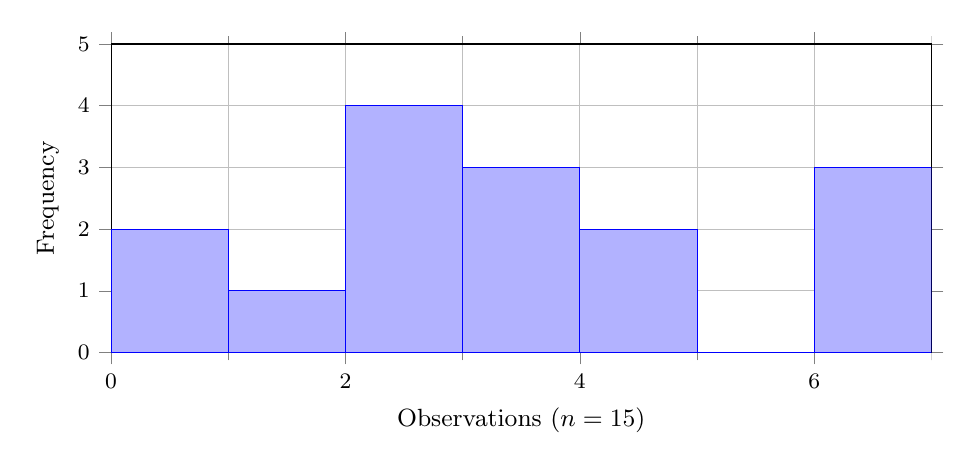
\begin{tikzpicture}
        \begin{axis}[
            small,
            height=5.5cm,
            width=12.0cm,
            enlarge x limits=false,
            enlarge y limits=false,
            %ybar interval,
            grid=both,
            %minor y tick num=1,
            minor x tick num=1,
            ylabel={Frequency},
            xlabel={Observations ($n=15$)},
            %x tick label style={rotate=0,anchor=south east},
            tick align=outside, % <-- this positions the ticks "outside"
            xtick={0, 2, 4,...,30},
            ytick={0, 1,...,30},
            ymin=0,
            ymax=5,
            xmin=0,
            xmax=7,
            xticklabel style={/pgf/number format/.cd,fixed,precision=0},
            xticklabel=
            \pgfmathprintnumber\tick,%--\pgfmathprintnumber\nexttick\%,
          ]
          \draw [blue,fill=blue!30!white] (axis cs: 0,0) rectangle (axis cs: 1,2);
          \draw [blue,fill=blue!30!white] (axis cs: 1,0) rectangle (axis cs: 2,1);
          \draw [blue,fill=blue!30!white] (axis cs: 2,0) rectangle (axis cs: 3,4);
          \draw [blue,fill=blue!30!white] (axis cs: 3,0) rectangle (axis cs: 4,3);
          \draw [blue,fill=blue!30!white] (axis cs: 4,0) rectangle (axis cs: 5,2);
          \draw [blue,fill=blue!30!white] (axis cs: 5,0) rectangle (axis cs: 6,0);
          \draw [blue,fill=blue!30!white] (axis cs: 6,0) rectangle (axis cs: 7,3);
        \end{axis}
      \end{tikzpicture}
    \end{center}

    \vspace{-4mm}
    \question{Is the normality condition met?}\pause
    \answer{Since there are less than 30 observations, we need to look for \emph{clear} outliers. While there is a gap on the right, the gap is small and 20\% of the observations fall in rightmost bar. We can't really call these clear outliers, so the normality condition is reasonably met.}
  \end{example}
\end{frame}

\begin{frame}
  \begin{example}
    \begin{center}
      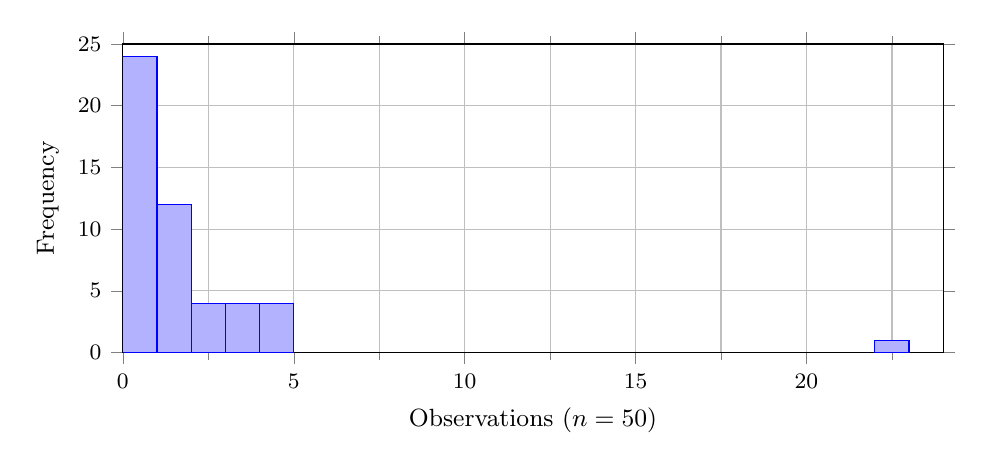
\begin{tikzpicture}
        \begin{axis}[
            small,
            height=5.5cm,
            width=12.0cm,
            enlarge x limits=false,
            enlarge y limits=false,
            %ybar interval,
            grid=both,
            %minor y tick num=1,
            minor x tick num=1,
            ylabel={Frequency},
            xlabel={Observations ($n=50$)},
            %x tick label style={rotate=0,anchor=south east},
            tick align=outside, % <-- this positions the ticks "outside"
            xtick={0, 5, 10,...,30},
            ytick={0, 5,...,30},
            ymin=0,
            ymax=25,
            xmin=0,
            xmax=24,
            xticklabel style={/pgf/number format/.cd,fixed,precision=0},
            xticklabel=
            \pgfmathprintnumber\tick,%--\pgfmathprintnumber\nexttick\%,
          ]
          \draw [blue,fill=blue!30!white] (axis cs: 0,0) rectangle (axis cs: 1,24);
          \draw [blue,fill=blue!30!white] (axis cs: 1,0) rectangle (axis cs: 2,12);
          \draw [blue,fill=blue!30!white] (axis cs: 2,0) rectangle (axis cs: 3,4);
          \draw [blue,fill=blue!30!white] (axis cs: 3,0) rectangle (axis cs: 4,4);
          \draw [blue,fill=blue!30!white] (axis cs: 4,0) rectangle (axis cs: 5,4);
          \draw [blue,fill=blue!30!white] (axis cs: 22,0) rectangle (axis cs: 23,1);
        \end{axis}
      \end{tikzpicture}
    \end{center}

    \vspace{-4mm}
    \question{Is the normality condition met?}\pause
    \answer{The sample size is greater than 30, so we need to look for an extreme outlier. The gap is more than four times the width of the cluster on the left side, so this is clearly an extreme outlier and the normality condition is not met.}
  \end{example}
\end{frame}

\begin{frame}
  \begin{note}
    In practice, we cannot directly calculate the standard error for $\bar{x}$, since we do not know the population standard deviation $\sigma$.\pause

    \vspace{1mm}
    We can use the sample standard deviation $s$ as the best estimate of $\sigma$:

    \vspace{-2mm}
    \begin{equation*}
      \begin{aligned}
        SE = \dfrac{\sigma}{\sqrt{n}}\approx\dfrac{s}{\sqrt{n}}
      \end{aligned}
    \end{equation*}
  \end{note}\pause
  
  \begin{definition}
    If a population has a normal distribution, then the distribution of 
    \begin{equation*}
      t = \dfrac{\bar{x}-\mu}{SE} \approx \dfrac{ \bar{x}-\mu }{ \dfrac{s}{ \sqrt{n} } }
    \end{equation*}
    is called the \textbf{Student $\boldsymbol{t}$ distribution} for sample sizes $n$.
  \end{definition}\pause

  \begin{note}
    A Student $t$ distribution is commonly called a \textbf{$\boldsymbol{t}$ distribution}.
  \end{note}
\end{frame}

\begin{frame}
  \begin{definition}
    The \textbf{degrees of freedom} (or \textbf{df}) for a collection of sample data is the number of sample values that can vary after certain restrictions have been imposed on all data values.

    \vspace{1mm}
    When modeling $\bar{x}$ using the $t$-distribution, use:

    \vspace{-4mm}
    \begin{equation*}
      df = n-1
    \end{equation*}
  \end{definition}\pause

  \begin{example}
    If 10 test scores must have mean 80, then their sum must be 800.\pause

    \vspace{2mm}
    We can freely assign values to the first 9 scores, but the 10th score would need to be:

    \vspace{-4mm}
    \begin{equation*}
      \text{s}_{10} = 800 - \text{s}_1 - \text{s}_2 - \text{s}_3 - \text{s}_4 - \text{s}_5 - \text{s}_6 - \text{s}_7 - \text{s}_8 - \text{s}_9
    \end{equation*}\pause

    \vspace{-4mm}
    Hence 9 degrees of freedom.
  \end{example}
\end{frame}

\begin{frame}[fragile]
  \begin{note}
    The Student $t$ distribution changes for different degrees of freedom.

    \vspace{1mm}
    \begin{overprint}
      \onslide<1 | handout:0>
      \begin{center}
        \begin{asy}
          size(200,95, IgnoreAspect);

          real xmin = -3.5; real xmax = 3.5;

          draw(normal_dist(0,1,xmin,xmax), black+dashed, "Std Normal");

          draw(t_dist(8, xmin, xmax), invisible, "$\phantom{df=8}$");
          draw(t_dist(4, xmin, xmax), invisible, "$\phantom{df=4}$");
          draw(t_dist(2, xmin, xmax), invisible, "$\phantom{df=2}$");
          draw(t_dist(1, xmin, xmax), invisible, "$\phantom{df=1}$");

          xaxis(RightTicks(new real[] {0}));

          attach(legend(), truepoint(E), 10E, UnFill);
        \end{asy}
      \end{center}
      \onslide<2 | handout:0>
      \begin{center}
        \begin{asy}
          size(200,95, IgnoreAspect);

          real xmin = -3.5; real xmax = 3.5;

          draw(normal_dist(0,1,xmin,xmax), black+dashed, "Std Normal");

          draw(t_dist(8, xmin, xmax), invisible, "$\phantom{df=8}$");
          draw(t_dist(4, xmin, xmax), invisible, "$\phantom{df=4}$");
          draw(t_dist(2, xmin, xmax), invisible, "$\phantom{df=2}$");
          draw(t_dist(1, xmin, xmax), palered, "$df=1$");
          
          xaxis(RightTicks(new real[] {0}));

          attach(legend(), truepoint(E), 10E, UnFill);
        \end{asy}
      \end{center}
      \onslide<3 | handout:0>
      \begin{center}
        \begin{asy}
          size(200,95, IgnoreAspect);

          real xmin = -3.5; real xmax = 3.5;

          draw(normal_dist(0,1,xmin,xmax), black+dashed, "Std Normal");

          draw(t_dist(8, xmin, xmax), invisible, "$\phantom{df=8}$");
          draw(t_dist(4, xmin, xmax), invisible, "$\phantom{df=4}$");
          draw(t_dist(2, xmin, xmax), lightred, "$df=2$");
          draw(t_dist(1, xmin, xmax), palered, "$df=1$");

          xaxis(RightTicks(new real[] {0}));

          attach(legend(), truepoint(E), 10E, UnFill);
        \end{asy}
      \end{center}
      \onslide<4 | handout:0>
      \begin{center}
        \begin{asy}
          size(200,95, IgnoreAspect);

          real xmin = -3.5; real xmax = 3.5;

          draw(normal_dist(0,1,xmin,xmax), black+dashed, "Std Normal");

          draw(t_dist(8, xmin, xmax), invisible, "$\phantom{df=8}$");
          draw(t_dist(4, xmin, xmax), red, "$df=4$");
          draw(t_dist(2, xmin, xmax), lightred, "$df=2$");
          draw(t_dist(1, xmin, xmax), palered, "$df=1$");
                
          xaxis(RightTicks(new real[] {0}));

          attach(legend(), truepoint(E), 10E, UnFill);
        \end{asy}
      \end{center}
      \onslide<5- | handout:1>
      \begin{center}
        \begin{asy}
          size(200,95, IgnoreAspect);

          real xmin = -3.5; real xmax = 3.5;

          draw(normal_dist(0,1,xmin,xmax), black+dashed, "Std Normal");

          draw(t_dist(8, xmin, xmax), heavyred, "$df=8$");
          draw(t_dist(4, xmin, xmax), red, "$df=4$");
          draw(t_dist(2, xmin, xmax), lightred, "$df=2$");
          draw(t_dist(1, xmin, xmax), palered, "$df=1$");
          
          xaxis(RightTicks(new real[] {0}));

          attach(legend(), truepoint(E), 10E, UnFill);
        \end{asy}
      \end{center}
    \end{overprint}
  \end{note}

  \onslide<6->
  \begin{note}
    The $t$-distribution has a mean of $t=0$ 

    \vspace{1mm}
    The standard deviation varies with $n$, but is always greater than 1.
  \end{note}

  \onslide<7->
  \begin{note}
    As the sample size gets larger, the Student $t$ distribution gets closer to the standard normal distribution.
  \end{note}
\end{frame}

\begin{frame}[fragile]
  \begin{example}
    The $t$-distribution with 13 degrees of freedom is shown.

    \vspace{1mm}
    \begin{overprint}
      \onslide<1 | handout: 0>
      \begin{center}
        \begin{asy}
          size(250,95, IgnoreAspect);

          real xmin = -5; real xmax = 5;

          real df = 13;

          draw(normal_dist(0,1,xmin,xmax), invisible);
          draw(t_dist(df, xmin, xmax), black);
          
          xaxis(RightTicks(new real[] {0, 1, -1, 2, -2, 3, -3, 4, -4}));
        \end{asy}
      \end{center}
      \onslide<2->
      \begin{center}
        \begin{asy}
          size(250,95, IgnoreAspect);

          real xmin = -5; real xmax = 5;

          real t = -2.10;
          real df = 13;

          draw(normal_dist(0,1,xmin,xmax), invisible);
          draw(t_dist(df, xmin, xmax), black);
          shade_below(df, t, xmin, xmax);
          
          xaxis(RightTicks(new real[] {0, 1, -1, 2, -2, 3, -3, 4, -4}));
        \end{asy}
      \end{center}
    \end{overprint}
    \onslide<2->
    The area to the left of $t=-2.1$ is:

    \vspace{-4mm}
    \begin{equation*}
      \begin{aligned}
        \prob{t \leq 2.1} \approx 0.0279
      \end{aligned}
    \end{equation*}
  \end{example}
\end{frame}

\begin{frame}[fragile]
  \begin{example}
    The $t$-distribution with 20 degrees of freedom is shown.

    \vspace{1mm}
    \begin{overprint}
      \onslide<1 | handout: 0>
      \begin{center}
        \begin{asy}
          size(250,95, IgnoreAspect);

          real xmin = -5; real xmax = 5;

          real df = 20;

          draw(normal_dist(0,1,xmin,xmax), invisible);
          draw(t_dist(df, xmin, xmax), black);
          
          xaxis(RightTicks(new real[] {0, 1, -1, 2, -2, 3, -3, 4, -4}));
        \end{asy}
      \end{center}
      \onslide<2->
      \begin{center}
        \begin{asy}
          size(250,95, IgnoreAspect);

          real xmin = -5; real xmax = 5;

          real t = 1.65;
          real df = 20;

          draw(normal_dist(0,1,xmin,xmax), invisible);
          draw(t_dist(df, xmin, xmax), black);
          shade_above(df, t, xmin, xmax);
          
          xaxis(RightTicks(new real[] {0, 1, -1, 2, -2, 3, -3, 4, -4}));
        \end{asy}
      \end{center}
    \end{overprint}
    \onslide<2->
    The area to the right of $t=1.65$ is:

    \vspace{-4mm}
    \begin{equation*}
      \begin{aligned}
        \prob{t \geq 1.65} \approx 0.0573
      \end{aligned}
    \end{equation*}
  \end{example}
\end{frame}

\begin{frame}[fragile]
  \begin{example}
    The $t$-distribution with 2 degrees of freedom is shown.

    \vspace{1mm}
    \begin{overprint}
      \onslide<1 | handout: 0>
      \begin{center}
        \begin{asy}
          size(250,95, IgnoreAspect);

          real xmin = -5; real xmax = 5;

          real df = 2;

          draw(normal_dist(0,1,xmin,xmax), invisible);
          draw(t_dist(df, xmin, xmax), black);
          
          xaxis(RightTicks(new real[] {0, 1, -1, 2, -2, 3, -3, 4, -4}));
        \end{asy}
      \end{center}
      \onslide<2->
      \begin{center}
        \begin{asy}
          size(250,95, IgnoreAspect);

          real xmin = -5; real xmax = 5;

          real t = 3;
          real df = 2;

          draw(normal_dist(0,1,xmin,xmax), invisible);
          draw(t_dist(df, xmin, xmax), black);
          shade_below(df, -t, xmin, xmax);
          shade_above(df, t, xmin, xmax);
          
          xaxis(RightTicks(new real[] {0, 1, -1, 2, -2, 3, -3, 4, -4}));
        \end{asy}
      \end{center}
    \end{overprint}
    \onslide<2->
    The area more than three units from the mean is:

    \vspace{-4mm}
    \begin{equation*}
      \begin{aligned}
        \prob{t \leq -3~\text{or}~t \geq 3} \approx 0.0955
      \end{aligned}
    \end{equation*}
  \end{example}
\end{frame}

\begin{frame}[fragile]
  \begin{example}
    Let us find the critical value, $t^*_{df}$, corresponding to a 95\% confidence level, given that the sample size is $n=15$.\pause

    \vspace{1mm}
    The degrees of freedom is $df=n-1\pause =15-1 =14$.\pause

    \vspace{1mm}
    We need to find the $t$-value that has $0.95+0.025=0.975$ to the left.

    \begin{center}
      \begin{asy}
        size(250,85, IgnoreAspect);

        real xmin = -4; real xmax = 4;

        real a = -2.145;
        real b = 2.145;

        guide g = t_dist(14, xmin, a);
        filldraw((xmin,0) -- g -- (a,0) -- cycle, orange, black);
        guide g = t_dist(14, b, xmax);
        filldraw((b,0) -- g -- (xmax,0) -- cycle, orange, black);
        guide g = t_dist(14, a, b);
        filldraw((a,0) -- g -- (b,0) -- cycle, yellow, black);
        draw(t_dist(14, xmin, xmax), black);

        label("0.95", (0, 0.5*pdf_tdist(0,14)));
        label("0.025", (a*1.1, pdf_tdist(a,14)), 3W);
        label("0.025", (b*1.1, pdf_tdist(b,14)), 3E);

        dot((b,0));
        label("$t^*_{14}$", (b,0), S);
        
        xaxis(RightTicks(new real[] {0}));
      \end{asy}
    \end{center}\pause

    \vspace{-2mm}
    Using technology we get $t^*_{14}=2.145$
  \end{example}\pause

  \begin{note}
    The critical value $t^*_{df}$ must be found every time, since the $t$-distribution changes for different sample sizes.
  \end{note}
\end{frame}

\begin{frame}
  \begin{block}{Confidence Interval For A Single Mean}
    \begin{description}
    \item[Prepare:] Identify $\bar{x}$, $s$, $n$, and what confidence level to use.\pause
    \item[Check:] Verify the conditions to ensure $\bar{x}$ is nearly normal:\pause
      \begin{itemize}
      \item The sample observations are nearly normal.\pause
      \item The population is normally distributed or $n\geq 30$.\pause
      \end{itemize}
    \item[Calculate:] If the conditions hold, compute:\pause
      \begin{itemize}
      \item The degrees of freedom: $df=n-1$\pause
      \item The critical value: $t^*_{df}$\pause
      \item The standard error: $SE=\dfrac{s}{\sqrt{n}}$\pause
      \item The confidence interval:

        \vspace{-4mm}
        \begin{equation*}
          \begin{aligned}
            \text{point estimate} \pm t^*_{df}\cdot SE\pause
            \quad\rightarrow\quad
            \bar{x} \pm t^*_{df}\cdot \dfrac{s}{\sqrt{n}}
          \end{aligned}
        \end{equation*}
      \end{itemize}\pause

      \vspace{-1mm}
    \item[Conclude:] Interpret the confidence interval in the context of the problem.
    \end{description}
  \end{block}
\end{frame}

\begin{frame}
  \begin{example}
    The weights (in hectograms, hg) of randomly selected girls at birth are

    \vspace{-7mm}
    \begin{center}
      {%
      \vspace{4.5mm}
      \setlength{\tabcolsep}{.4em}
      \begin{tabular}{ccccccccccccccc}
        33 & 28 & 33 & 37 & 31 & 32 & 31 & 28 & 34 & 28 & 33 & 26 & 30 & 31 & 28
      \end{tabular}
      }
    \end{center}

    \vspace{-3mm}
    (Based on data from the National Center for Health Statistics.)\pause

    \vspace{1mm}
    The summary statistics for this sample are
    \vspace{-3mm}
    \begin{equation*}
      n = 15
      \qquad\qquad \bar{x} = 30.9
      \qquad\qquad s  = 2.9
    \end{equation*}\pause

    \vspace{-8mm}
    Construct a 95\% confidence interval for the mean birth weight of girls.\pause

    \vspace{1mm}
    The margin of error is

    \vspace{-3mm}
    \begin{equation*}
      E=t^*_{14}\cdot\dfrac{s}{\sqrt{n}}\pause
      =2.145\cdot\dfrac{2.9}{\sqrt{15}}\pause
      =1.606126
    \end{equation*}\pause

    \vspace{-4mm}
    The confidence interval is

    \vspace{-3mm}
    \begin{equation*}
      \begin{matrix}
        \bar{x} - E &<& \mu &<& \bar{x} + E\\\pause
        30.9 - 1.606126 &<& \mu &<& 30.9 + 1.606126 \\\pause
        29.3~\text{hg} &<& \mu &<& 32.5~\text{hg} \\
      \end{matrix}
    \end{equation*}\pause

    \vspace{-3mm}
    We are 95\% confident that the interval from 29.2 hg to 32.5 hg actually does contain the true value of $\mu$.
  \end{example}
\end{frame}

\begin{frame}
  \begin{block}{Hypothesis Testing For A Single Mean}
    \begin{description}
    \item[Prepare:] Identify the parameter of interest, list out hypotheses, identify $\bar{x}$, $s$, $n$, and what confidence level to use.\pause
    \item[Check:] Verify the conditions to ensure $\bar{x}$ is nearly normal:\pause
      \begin{itemize}
      \item The sample observations are nearly normal.\pause
      \item The population is normally distributed or $n\geq 30$.\pause
      \end{itemize}
    \item[Calculate:] If the conditions hold, compute:\pause
      \begin{itemize}
      \item The degrees of freedom: $df=n-1$\pause
      \item The standard error: $SE=\dfrac{s}{\sqrt{n}}$\pause
      \item The $t$-score: $t = \dfrac{\bar{x} - \text{null value}}{SE}$\pause
      \item The $p$-value.\pause
      \end{itemize}
    \item[Conclude:] Evaluate the hypothesis test by comparing the $p$-value to $\alpha$, and provide a conclusion in the context of the problem.
    \end{description}
  \end{block}
\end{frame}

\begin{frame}
  \begin{example}
    The Cheery Blossom Race is a 10-mile race in Washington, D.C. held every spring.\pause

    \vspace{1mm}
    The average time for all runners who finished the Cherry Blossom Race in 2006 was 93.29 minutes.\pause

    \vspace{1mm}
    We want to determine using data from 100 participants in the 2017 Cherry Blossom Race whether runners are getting faster or slower.\pause

    \vspace{1mm}
    \question{What are the null and alternative hypotheses?}\pause
    \answer{%

      \vspace{-8mm}
      \begin{equation*}
        \begin{aligned}
          H_0: & \text{The average time was the same in 2007 and 2017}\\
          &\mu=93.29 \\
          H_A: & \text{The average time was different in 2017 compared to 2007}\\
          &\mu\neq93.29
        \end{aligned}
      \end{equation*}
    }

    \vspace{-4mm}
  \end{example}
\end{frame}

\begin{frame}
  \begin{examplecont}
    The histogram shows the times for 100 of the runners in the 2017 race.

    \vspace{-6mm}
    \begin{center}
      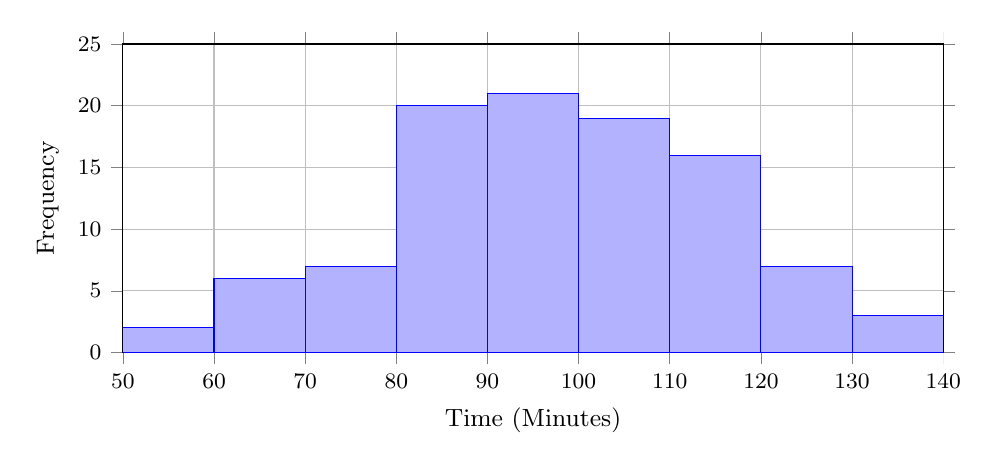
\begin{tikzpicture}
        \begin{axis}[
            small,
            height=5.5cm,
            width=12.0cm,
            enlarge x limits=false,
            enlarge y limits=false,
            %ybar interval,
            grid=both,
            %minor y tick num=1,
            %minor x tick num=1,
            ylabel={Frequency},
            xlabel={Time (Minutes)},
            %x tick label style={rotate=0,anchor=south east},
            tick align=outside, % <-- this positions the ticks "outside"
            xtick={0, 10,...,300},
            ytick={0, 5,...,300},
            ymin=0,
            ymax=25,
            xmin=50,
            xmax=140,
            xticklabel style={/pgf/number format/.cd,fixed,precision=0},
            xticklabel=
            \pgfmathprintnumber\tick,%--\pgfmathprintnumber\nexttick\%,
          ]
          \draw [blue,fill=blue!30!white] (axis cs: 50,0) rectangle (axis cs: 60,2);
          \draw [blue,fill=blue!30!white] (axis cs: 60,0) rectangle (axis cs: 70,6);
          \draw [blue,fill=blue!30!white] (axis cs: 70,0) rectangle (axis cs: 80,7);
          \draw [blue,fill=blue!30!white] (axis cs: 80,0) rectangle (axis cs: 90,20);
          \draw [blue,fill=blue!30!white] (axis cs: 90,0) rectangle (axis cs: 100,21);
          \draw [blue,fill=blue!30!white] (axis cs: 100,0) rectangle (axis cs: 110,19);
          \draw [blue,fill=blue!30!white] (axis cs: 110,0) rectangle (axis cs: 120,16);
          \draw [blue,fill=blue!30!white] (axis cs: 120,0) rectangle (axis cs: 130,7);
          \draw [blue,fill=blue!30!white] (axis cs: 130,0) rectangle (axis cs: 140,3);
        \end{axis}
      \end{tikzpicture}
    \end{center}

    \vspace{-2mm}
    \question{Is the normality condition satisfied?}\pause
    \answer{We have more than 30 observations and there are no outliers, so yes.}
  \end{examplecont}
\end{frame}

\begin{frame}
  \begin{examplecont}
    In 2007, the average time was 93.29 minutes. Our sample of 100 runners from 2017 have a mean of 97.32 minutes and standard deviation of 16.98 minutes.\pause

    \vspace{1mm}
    The degrees of freedom are $df=n-1\pause =100-1=99$.\pause

    \vspace{1mm}
    The standard error is:
    \begin{equation*}
      \begin{aligned}
        SE &= \dfrac{s}{\sqrt{n}}\pause = \dfrac{16.98}{\sqrt{100}} = 1.70
      \end{aligned}
    \end{equation*}\pause

    \vspace{-6mm}
    The $t$-score is:
    \begin{equation*}
      \begin{aligned}
        t = \dfrac{\bar{x} - \text{null value}}{SE}\pause = \dfrac{97.32-93.29}{1.70} = 2.37
      \end{aligned}
    \end{equation*}
  \end{examplecont}
\end{frame}

\begin{frame}[fragile]
  \begin{examplecont}
    So, we wish to find the area of the tails:
    \begin{center}
        \begin{asy}
          size(250,90, IgnoreAspect);

          real xmin = -5; real xmax = 5;

          real t = 2.37;
          real df = 99;

          draw(t_dist(df, xmin, xmax), black);
          shade_below(df, -t, xmin, xmax, red);
          shade_above(df, t, xmin, xmax, red);
          
          xaxis(RightTicks(new real[] {0, 1, -1, 2, -2, 3, -3, 4, -4}));
        \end{asy}
    \end{center}\pause

    Using technology, we get a $p$-value of 0.02.\pause

    \vspace{1mm}
    \question{Do we reject or fail to reject $H_0$?}\pause
    \answer{Because $0.02 < 0.05$, we reject the null hypothesis.}\pause

    \vspace{1mm}
    Because we reject the null hypothsis, we have evidence that there is a difference in average race times between the 2007 and 2017 races.\pause

    \vspace{1mm}
    Since the average in 2017 (97.32 minutes) is larger than the average in 2007 (93.29 minutes), it is likely that racers in 2017 were slower.
  \end{examplecont}
\end{frame}
\end{document}
